\documentclass{beamer}
\usepackage{graphicx}
\usepackage{hyperref}

\usetheme{Execushares}

\begin{document}
\title{Project Proposal: MorphCore}
\subtitle{Amanda Marano, Brian Jacobs, Pete Ehrett}
\author{Team DRRA}
\date{\today}

\frame{\titlepage}

\frame{
  \frametitle{Project Overview}
  \begin{itemize}
    \item Build a MorphCore processor
    \item Put Linux on it
    \item Run something cool
  \end{itemize}
  \hfill 
  \begin{tabular}{c}
    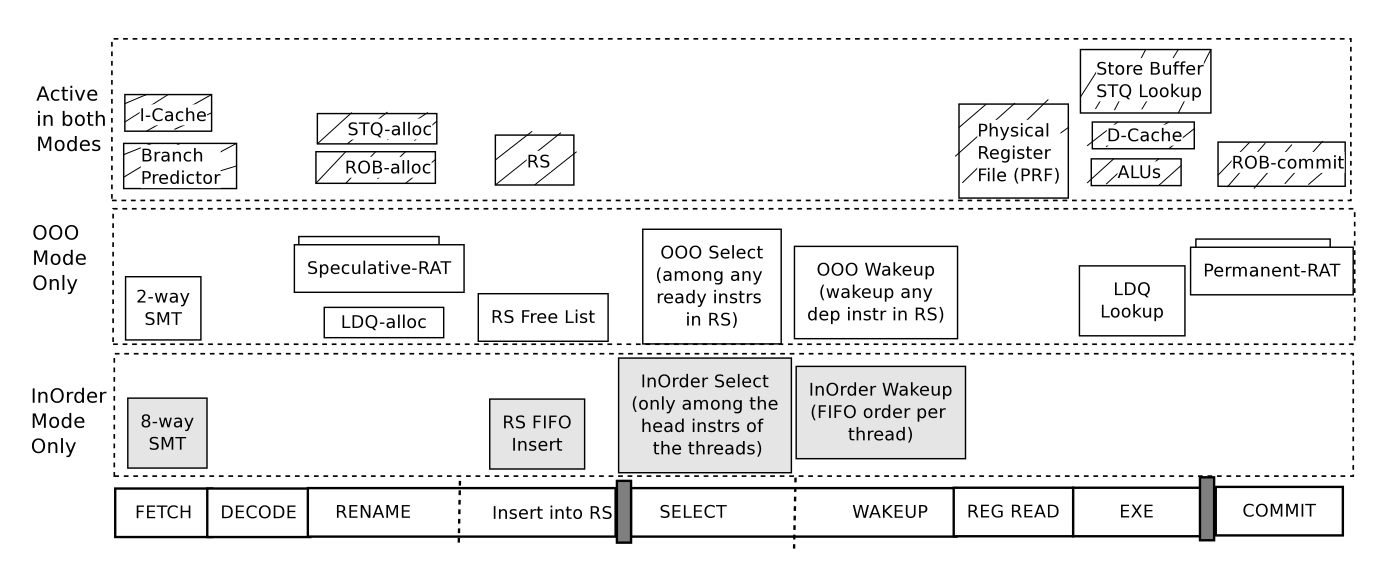
\includegraphics[width=3in]{Morph.png}\\
    \textit{\tiny MorphCore Microarchitecture from the MorphCore paper}
  \end{tabular}
}

\frame{
  \frametitle{MorphCore}
  \begin{itemize}
    \item Two operating modes: OutOfOrder, InOrder
    \item Swaps between instruction level parallelism and thread level parallelism
    \item Uses same hardware in different configurations
    \item OutOfOrder is a single OOO core
    \item InOrder is a set of multiple in-order cores
    \item Described in the paper:
  \end{itemize}
  \vspace{-.2in}
  \begin{center}
    \textbf{MorphCore: An Energy-Efficient Microarchitecture for}\\
    \textbf{High Performance ILP and High Throughput TLP}\\

    Khubaib \hspace{.25in} M.~Aater~Suleman \hspace{.25in} Milad~Hashemi \hspace{.25in} Chris~Wilkerson \hspace{.25in} Yale~N.~Patt 
  \end{center}
}

\frame{
  \frametitle{Potential Pitfalls}
  \begin{itemize}
    \item Running Linux means we'd need things to be VERY correct.
      \begin{itemize}
        \item Verify, verify, verify!
      \end{itemize}
    \item Building an OOO cpu is a substantial undertaking, which could be hard to get working.
    \item The MorphCore is not a common design---resources could be more difficult to come by.
    \item The existing ARM core design, the Amber core from OpenCores \raisebox{.1em}{\tiny(\url{http://opencores.org/project,amber,Overview})} might be difficult to work with.
  \end{itemize}
}

\frame{
  \frametitle{Project Timeline}
  \begin{itemize}
    \item Verify existing ARM core
      \begin{itemize}
        \item Design some tests, ideally with good coverage, which can transfer over to other ARM implementations.
      \end{itemize}
    \item Convert the ARM core to Out of Order
      \begin{itemize}
        \item This is likely the bulk of the work.
      \end{itemize}
    \item Other hardware necessary to demo. Can be parallel with other development.
      \begin{itemize}
        \item VGA driver
        \item Sound driver
      \end{itemize}
    \item Multicore the OOO ARM.
      \begin{itemize}
        \item This is also a substantial amount of work.
      \end{itemize}
  \end{itemize}
}

\frame{
  \frametitle{Platform Choice}
  \begin{itemize}
    \item ZedBoard FPGA?
  \end{itemize}
  \vspace{-.2in}
  \begin{center}
    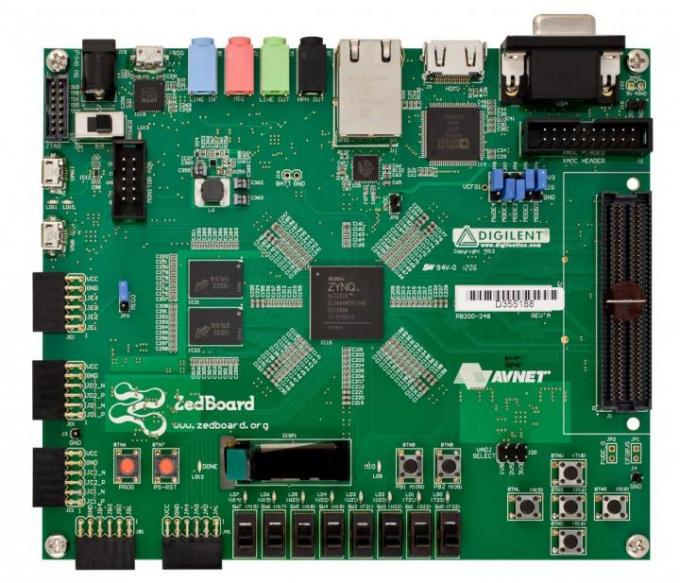
\includegraphics[width=1.5in]{ZedBoard.jpg}
  \end{center}
  \vspace{-.2in}
  \begin{itemize}
    \item ARM Cores could be useful if we run into problems with our FPGA ARM.
    \item Downside: Toolchain is extremely unwieldy.
  \end{itemize}
  \begin{center}
    \textcolor{green}{\Huge\bf YES}
  \end{center}
}

\frame{
  \frametitle{Success Criteria}

  \colorlet{originalText}{ExecusharesBlack}
  \colorlet{originalBullet}{ExecusharesBlue}

  \def\updateColors{
      \colorlet{ExecusharesBlue}{ExecusharesBlue!60!white}
      \colorlet{ExecusharesBlack}{ExecusharesBlack!60!white}
  }

  \begin{itemize}
    \item \textcolor{ExecusharesBlack}{100\% Success: Linux runs on a MorphCore, we can demo some sort of simple game with graphics and sound.}
      \updateColors
    \item \textcolor{ExecusharesBlack}{90\% Success: We can demo both in-order multicore and OOO single-core running Linux, but without MorphCore.}
      \updateColors
    \item \textcolor{ExecusharesBlack}{Mostly Successful: The OOO modifications work, we can run Linux, same demo.}
      \updateColors
    \item \textcolor{ExecusharesBlack}{Well, it works: Some code of some sort running on the OOO ARM core.}
      \updateColors
    \item \textcolor{ExecusharesBlack}{Not Successful: ``Something works.''}
      \updateColors
    \item \textcolor{ExecusharesBlack}{Failure: lawsuit(s) and/or injury}
  \end{itemize}

  \colorlet{ExecusharesBlack}{originalText}
  \colorlet{ExecusharesBlue}{originalBullet}
}

\end{document}